\section{Design}

\begin{figure}[h]
    \centering
    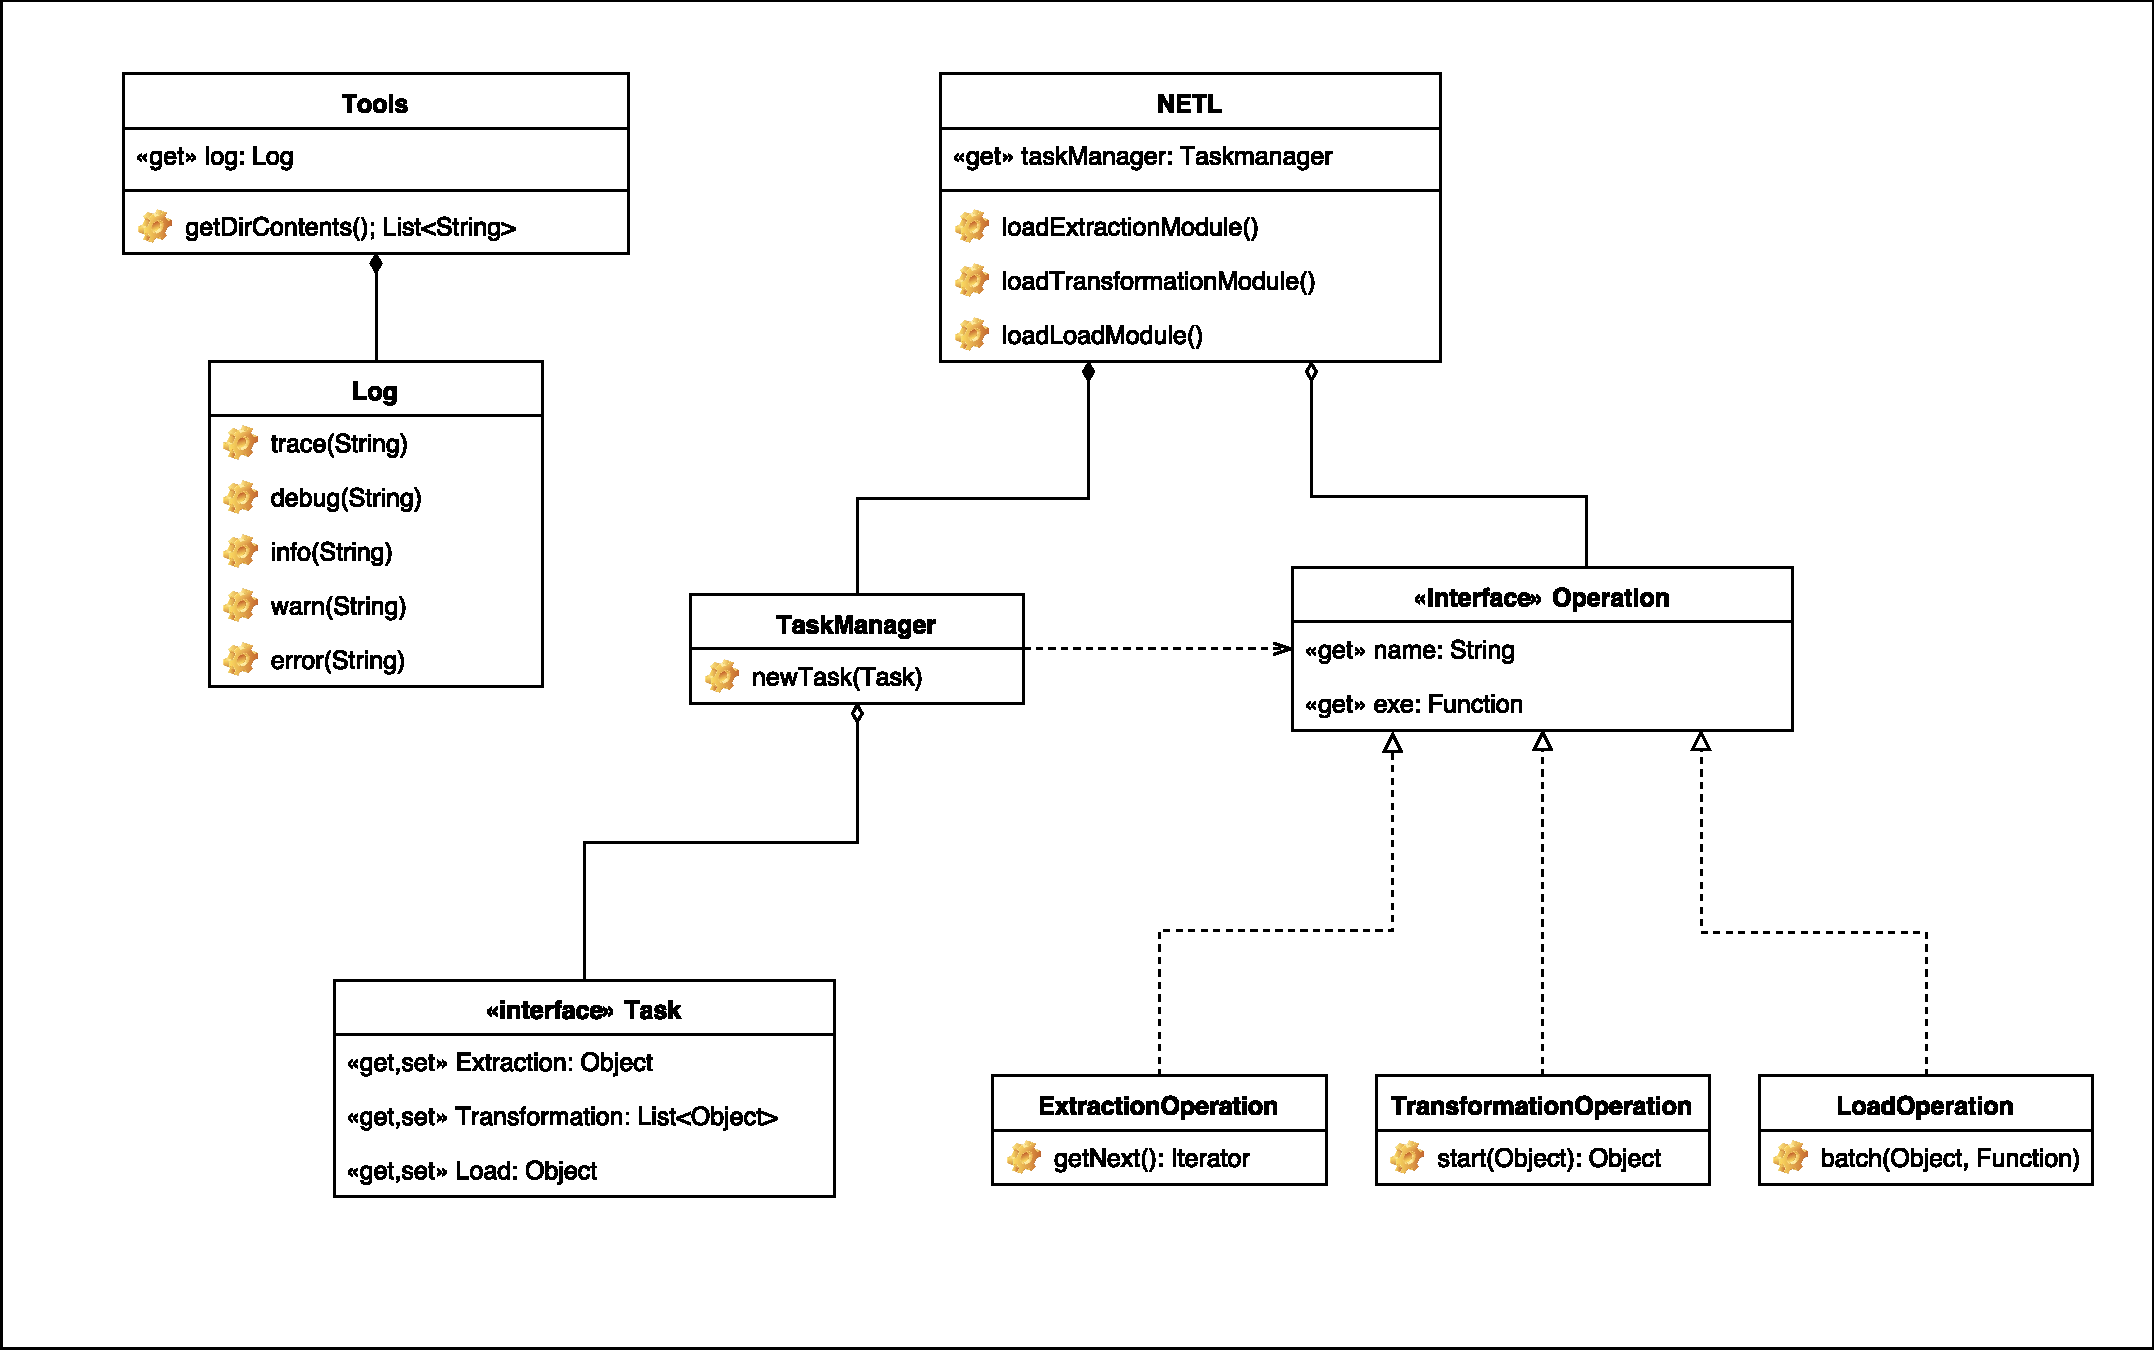
\includegraphics[scale=0.4]{./resources/figures/netlUML}
    \caption[nETL]{nETL}
    \label{nETL}
\end{figure}

Figure \ref{nETL} shows a potential architecture for a configurable component-based ETL tool. The intention of the framework is that it works on the basis of a pipeline of tasks. These tasks can be divided into 3 steps; an extraction step, a transformation step and a loading step. xxx insert something about ETL variations and why I chose the ETL pipeline.

\begin{enumerate}
    \item Extract data from a source specified by a user into memory
    \item Apply any number of transformations to the data in memory
    \item Load the data from memory into a destination specified by a user
\end{enumerate}

The framework itself is quite lightweight and comprises just the NETL, TaskManager and general purpose 'Tools' classes. For the purposes of this thesis, the framework as described by Figure \ref{nETL} has been prototyped in node.js with the source code available at xxx (there is also an npm package available at xxx). JavaScript is a suitable language to prototype this application for a number of reasons:

\begin{enumerate}
    \item It has a very succinct API making it fast to write code in (i.e. it is a highly abstracted language similarly to Ruby or Python)
    \item But unlike Ruby or Python (and other high level languages), it is opinionated in that it handles IO asynchronously by default
    \item The JavaScript implementation of object-orientation allows for easy runtime manipulation of the object model
    \item Another reason for choosing JavaScript is that it is very much in line with the spirit of CouchDB and the web in general
\end{enumerate}

nETL is primarily a task-managing application, and as such, the TaskManager class is effectively the core of the application. It is intended that it can be instantiated as an instance (i.e. there can be many TaskManager instances hosted within a single running application). In JavaScript this is best implemented via a constructor:

\begin{minted}{javascript}
/* File taskmanager.js */
function TaskManager(extractions, transformations, loads) {
    this.tasks = {};

    // Hold references to extractions/transformation/loads of the main application process
    this.extractions = extractions;
    this.transformations = transformations;
    this.loads = loads;
};

TaskManager.prototype.newTask = function(task) {
    // Add task to this.tasks and execute the task
};

module.exports = TaskManager;
\end{minted}

The application itself is intended to be singleton instance of \mintinline{javascript}{class NETL{}}, which provides an IO interface (either a console terminal or otherwise) to TaskManager instances, and modular extraction/transformation and load operations. Singleton's are typically implemented via the modular pattern in JavaScript, which is typically how libraries are delivered to users by package managers and invoked by \mintinline{javascript}{var library = require('library-name')();}. One possible way of implementing the NETL class in JavaScript (i.e the method that is used within this project's code base) is shown here:

\begin{minted}{javascript}
/* File netl.js */
module.exports = function() {
    // Private properties / methods
    const _extractions = {};
    const _transformations = {};
    const _loads = {};        
    const _taskManager = new TaskManager(_extractions, _transformations, _loads);
    function _loadExtractionModule(extractionOperation){};
    function _loadTransformationModule(transformOperation){};
    function _loadLoadModule(loadOperation){};

    // Make process API available
    return {
        taskManager: _taskManager,
        loadExtractionModule: _loadExtractionModule,
        loadTransformationModule: _loadTransformationModule,
        loadLoadModule: _loadLoadModule
    };
};
\end{minted}